\documentclass{article}
\usepackage{microtype}
\usepackage{graphicx}
\usepackage{booktabs}
\usepackage{hyperref}
\usepackage{amsmath,amssymb,amsthm}
\usepackage[accepted]{icml2025}
\newtheorem{theorem}{Theorem}
\newtheorem{lemma}[theorem]{Lemma}
\icmltitlerunning{Deadline-Aware Serving of LLM Agent Workloads (Midterm Report)}

\begin{document}
\twocolumn[
\icmltitle{Deadline-Aware Serving of LLM Agent Workloads:\\Batching, KV Caching, and Asynchronous Tool Calls}
\begin{icmlauthorlist}
\icmlauthor{[Author names]}{h}
\end{icmlauthorlist}
\icmlaffiliation{h}{Harvard University, CS 243 (Fall 2026). Midterm report}
\icmlcorrespondingauthor{[Author]}{[email]}
\icmlkeywords{LLM serving, agents, scheduling, KV cache, online algorithms}
\vskip 0.3in
]
\printAffiliationsAndNotice{}

\begin{abstract}
LLM agents interleave model calls with tool calls of unpredictable latency, and many agents, sometimes
collaborating on one task, share one GPU. Each serving decision then affects every task's deadline: which
requests to batch, which KV caches to keep, evict or preload, and whether a tool call blocks the agent or runs
asynchronously. We formulate this as one online scheduling problem. We prove it NP-hard even in a trivial
special case, so we target a constant-factor online algorithm, and we prove the first two reductions toward
it: continuous batching is equivalent, up to a factor of 2 in speed, to a set of identical parallel machines,
and issuing tool calls eagerly never hurts the optimum. All proofs are machine-checked (Z3 for the algebra,
exhaustive and randomized tests for the combinatorics). On the systems side we built a deadline-enforcing
agent runtime on vLLM and measured its first slice on an A40: asynchronous tool calls with KV
\emph{preloading}, which prefills tool results into the prefix cache while other tools are still running. On
20 held-out multi-hop questions with 8 parallel searches, preloading finished every task earlier (1.6\,s on
average, 95\% CI 1.49--1.72) with identical answers, and cut deadline misses at 16\,s from 45\% to 15\%.
\end{abstract}

\section{Problem}
\label{sec:problem}
Agents issue tool calls (search, code execution, APIs, other agents) whose latency is long and random compared
with a model step, often several in parallel~\cite{kim2024llmcompiler}. Deployments put many agents on one
GPU (setting a), and one task may itself be several collaborating agents, such as an orchestrator with
sub-agents (setting b). Under end-to-end deadlines the serving layer faces coupled decisions:
\textbf{batching} (running requests together raises throughput but slows each one), \textbf{KV memory} (keep a
paused agent's cache through a tool wait, evict it and recompute later, or prefill tool results before they
are needed), and \textbf{tool-call execution} (block the agent on a call, or continue and consume the result
later).

\textbf{Why it is new.} Existing systems address pieces: vLLM~\cite{kwon2023vllm} and
SGLang~\cite{zheng2024sglang} batch requests and reuse prefixes, InferCept~\cite{abhyankar2024infercept}
manages KV caches of requests paused for external calls, and Parrot~\cite{lin2024parrot} schedules multi-call
LLM applications. None decides batching, KV and tool execution jointly against task deadlines, and none gives
guarantees. Our goal is an online algorithm with a provable constant-factor guarantee, implemented as a layer on
vLLM.

\textbf{Challenges.} Tool durations and output lengths are unknown when decisions are made; GPU time and KV
memory are coupled (eviction saves memory but costs recompute); and deadlines belong to tasks, not to the
individual model calls the engine sees.

\section{Model and theory}
\label{sec:theory}
\textbf{Model.} One GPU runs an iteration-level batching engine. A decode step with $B$ running sequences takes
$\tau(B)=a+cB$ seconds; KV memory holds $M$ tokens. Task $j$ arrives at $r_j$ with deadline $d_j$ and value
$w_j$, and is a DAG of LLM nodes (model calls by any of its agents) and tool nodes (off-GPU calls with random
durations). A tool result may be consumed at any later LLM node of its agent that the program allows
(synchronous = the next node). Online, without knowing future arrivals, durations or output lengths, the
runtime chooses batches, KV keep/evict/preload actions, and tool issue and consumption points, to maximize the
total value of tasks finished by their deadlines. The full model is in the project documentation.

\begin{theorem}[NP-hardness]
The offline problem is NP-hard even with batch size 1, no tools, unlimited KV memory, deterministic lengths,
single-node tasks and $r_j=0$.
\end{theorem}
\begin{proof}[Proof sketch]
These restrictions give $1\,\|\,\sum w_jU_j$. With a common deadline equal to a knapsack capacity, $p_j$ = item
weight and $w_j$ = item value, a job set is on time iff its total length fits, so the problem is
Knapsack~\cite{karp1972}.
\end{proof}
With release dates and no preemption even unit values are strongly NP-hard~\cite{lenstra1977}, and online,
no deterministic algorithm on one machine guarantees more than $1/4$ of the optimum even when value is
proportional to work~\cite{baruah1992}; with unbounded value densities no constant ratio is
possible~\cite{koren1995}. Since the problem must be solved online anyway, \textbf{we target a constant-factor
competitive algorithm under resource augmentation}~\cite{kalyanasundaram2000}: the algorithm may use a
constant-factor faster GPU or larger KV memory than the optimum it is compared against. We reduce each
resource to a classical online problem.

\begin{lemma}[Batching $\to$ parallel machines]
If $m=a/c$ is an integer, (i) any schedule on $m$ identical machines of speed $1/(2a)$ (preemption, migration)
can be executed by the engine with no completion later, and (ii) any engine schedule can be executed on $m$
machines of speed $1/a$.
\end{lemma}
\begin{proof}
(i) At most $m$ jobs run, so $B\le a/c$ and each sequence advances at $1/(a+cB)\ge1/(2a)$. (ii) Each sequence
advances at $\le1/a$ and the batch at $B/(a+cB)<1/c=m/a$; such a rate vector is realizable on $m$ machines of
speed $1/a$ by McNaughton's wrap-around rule~\cite{mcnaughton1959}.
\end{proof}
Hence a $C$-competitive online algorithm for identical machines with speed augmentation $\sigma$ becomes
$C$-competitive on the engine with augmentation $2\sigma$ (a further factor $\le2$ if $a/c$ is not an integer
and $a\ge2c$).

\begin{lemma}[Eager asynchronous tool calls]
If tools share no capacity limit and their durations and results do not depend on issue or consumption time,
issuing every tool call as soon as its inputs exist never lowers the offline optimum.
\end{lemma}
\begin{proof}
Earlier issue only makes dependent nodes available earlier; every feasible schedule stays feasible.
\end{proof}
With eager issue, each task becomes a stream of LLM-node jobs released online, the setting of the remaining
steps: (1) per-node sub-deadlines from task deadlines and remaining critical paths, with deadline-ordered,
value-density-based admission on the machines of Lemma~2~\cite{koren1995}; (2) KV keep/evict as online caching
with variable sizes and recompute costs, where LRU-style and Landlord policies are 2-competitive with twice the
memory~\cite{sleator1985,young2002}, using the predicted tool return time as the next-use estimate; and (3) a
composition proof that charges eviction recompute to the speed augmentation.

\textbf{Verification.} Every algebraic step of Lemma~2 is proved with Z3 (the negation is unsatisfiable over the
reals; Z3 also finds a counterexample when the batch condition is dropped). Theorem~1, McNaughton's rule,
Lemma~2(i) and Lemma~3 are checked exhaustively on small instances and by randomized property tests, along with
a counterexample to Lemma~3 when tools share a slot (issue order then matters); 663 tests pass.

\begin{figure*}[t]
\centering
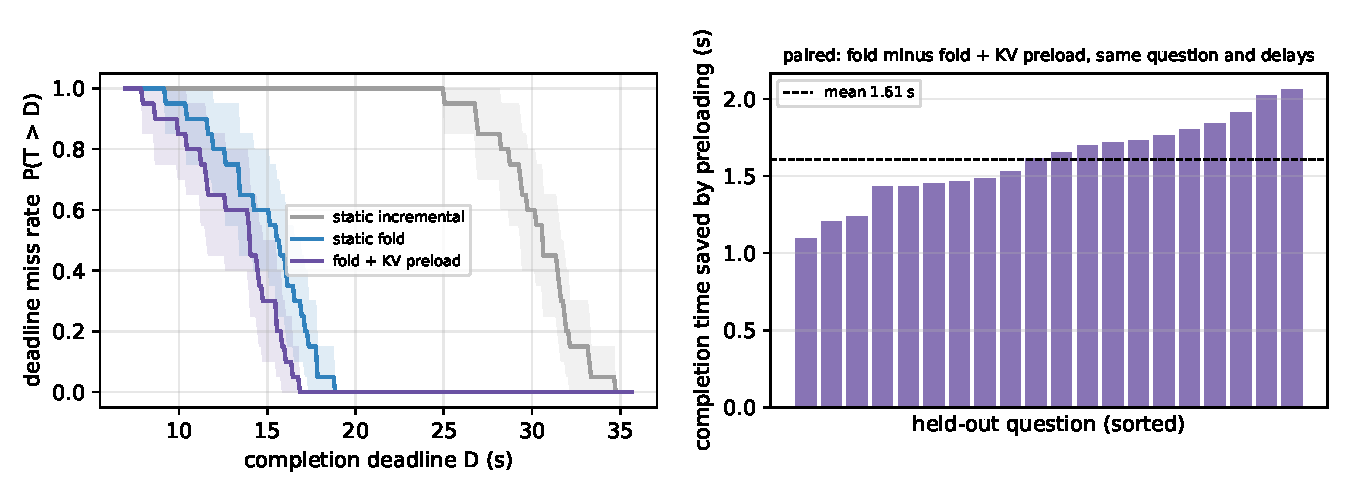
\includegraphics[width=0.78\textwidth]{figs/preload_load.pdf}
\vspace{-2mm}
\caption{\textbf{Asynchronous tool calls with KV preloading on vLLM} (20 held-out questions, 8 parallel
searches per question). Left: deadline miss rate $P(T>D)$ vs.\ deadline, 95\% bootstrap bands over questions.
Right: paired completion-time saving of preloading per question (same question, same tool delays).}
\label{fig:main}
\end{figure*}

\section{System}
\label{sec:system}
\textbf{Runtime.} A deadline-enforcing agent runtime in front of vLLM. Each task is an agent program (a single
agent that fans out parallel searches, or an orchestrator with worker agents); tool calls are issued
asynchronously as soon as their inputs exist (Lemma~3), and one timeout covers planning, tools, every model call
and the answer, cancelling outstanding work at the deadline. Every event is traced, and from the traces we
compute serving metrics (GPU busy and idle time during tool waits, prefill tokens computed vs.\ reused).

\textbf{Serving layer.} Many tasks share one vLLM server. For each model request the layer sets the engine
priority (FCFS; EDF by task deadline; or least laxity, i.e.\ the task deadline minus the estimated remaining
critical path) through vLLM's priority scheduling, and with admission control it drops a task whose estimated
finish, stretched by the current batch slowdown, is past its deadline. The same code runs against a simulated
continuous-batching engine (step time $a + cB$ plus prefill, KV capacity, priority queue) for CPU experiments.

\textbf{Cost model.} 48 profiled requests on the serving stack fit an affine model: 0.18\,ms per prefill
token, 29.3\,ms per decode token ($R^2=0.9999$, median error 0.4\%). Decoding with $B$ concurrent sequences
($B=1,\dots,128$) fits $\tau(B)=a+cB$ with $a=27.8$\,ms and $c=0.543$\,ms ($R^2=0.9992$, at most 3\% error per
point), so Lemma~2's $m=a/c\approx51$: batching up to ${\sim}51$ requests at most doubles each request's
per-token time.

\textbf{KV preloading.} The final prompt is an append-only log of tool results, so each \emph{preload}
request (the log so far, one output token) is a prefix of the final prompt and vLLM's automatic prefix caching
reuses its KV blocks. Preloads are charged to the deadline and issued only while tools are still running; the
cache is reset before every task so runs are independent.

\section{Initial evaluation}
\label{sec:eval}
\textbf{Setup.} Qwen3-8B~\cite{qwen3} on vLLM 0.32.0, one A40, one task at a time (the first slice of
setting a). Tasks are held-out HotpotQA questions~\cite{yang2018hotpotqa}. The agent plans 8 searches and
issues them asynchronously at once over a pooled corpus (the question's 10 paragraphs plus 90 distractor
paragraphs), top-10 passages each, ${\sim}$1.4k tokens per result and an ${\sim}$11k-token final prompt; no
context cap. Tool delays are reproducible draws (Uniform[0.5,4]\,s, or with probability 0.3 Uniform[4,12]\,s),
identical across policies. The policies compared never read the clock, so one run per question gives its
completion time $T$ and the miss rate at \emph{every} deadline $D$ is exactly $P(T>D)$ on the same runs.

\textbf{Result.} Preloading finished earlier on 20 of 20 questions, by 1.61\,s on average (95\% CI
1.49--1.72; range 1.10--2.06), with identical answers on all 20 (Figure~\ref{fig:main}). At $D=16$\,s the miss
rate fell from 0.45 to 0.15. Table~\ref{tab:serving} shows why: without preloading the GPU is idle for the whole
tool wait and the final request prefills ${\sim}$11k tokens after the last tool returns; with preloading,
87\% of the final prompt comes from the cache and the model time after the last return drops from 2.34\,s to
0.73\,s. Preloading is not free: 6.6 preload requests per task (median 0.32\,s each) used 2.2\,s of GPU time to
save 1.6\,s, which pays off only because that time was otherwise idle. In a multi-tenant setting it competes
with other agents, which is exactly the trade-off the general algorithm must make.

\begin{table}[t]
\centering
\caption{Serving view (means over the 20 questions). GPU util.\ = fraction of the tool-wait window in which the
model is busy; cached = share of the final request's prompt served from the prefix cache.}
\label{tab:serving}
\resizebox{\columnwidth}{!}{%
\begin{tabular}{lccccc}
\toprule
policy & end (s) & GPU util. & model s after & GPU s & cached \\
 & & during tools & last return & total & (final) \\
\midrule
wait for all, then answer & 14.86 & 0.00 & 2.34 & 6.1 & 0\% \\
+ KV preload & 13.26 & 0.28 & 0.73 & 6.6 & 87\% \\
\bottomrule
\end{tabular}}
\vspace{-3mm}
\end{table}

\textbf{Microbenchmark.} Isolating the final request (30 measurements), its latency without preloading grows
with evidence size (0.79\,s at 2.8k tokens, 2.29\,s at 10.8k) and stays at 0.39--0.51\,s with preloading, with
72--94\% of the prompt cached for 4--16 results (server-reported \texttt{cached\_tokens}). At small evidence
sizes the saving is small (0.15--0.3\,s at 2--3k tokens).

\textbf{Multi-tenant simulation (not GPU measurements).} On the simulated engine with the measured $c$
($c=0.5$\,ms; 3 seeds, 120\,s of Poisson arrivals, a mix of fan-out and orchestrator tasks, deadlines 1.5--4$\times$
the unloaded completion time), FCFS and EDF finish 96--98\% of tasks on time up to 1.5 tasks/s but fall to 0.57
at 3 tasks/s and 0.29 at 4 tasks/s. EDF alone does not help, because with up to 256 concurrent sequences requests
rarely wait in the engine queue. Admission control raises the on-time fraction to 0.73 and 0.55 by dropping
tasks that can no longer finish (21\% and 34\% of tasks). Running the same layer on the GPU is the next step.

\section{Remaining challenges and plan}
\label{sec:plan}
\textbf{Theory.} Prove the remaining steps of Section~\ref{sec:theory}: the sub-deadline assignment and its
loss, the KV caching reduction with recompute costs, and the composed constant-factor guarantee; extend
Lemma~2 to steps that mix prefill and decode. \textbf{System.} Run the multi-tenant layer on the GPU; implement the policy as a vLLM layer (request priorities and admission first, a scheduler change
only if needed), including KV keep/evict decisions during tool waits; add collaborating-agent tasks
(orchestrator and sub-agents) and the synchronous vs.\ asynchronous choice. \textbf{Evaluation.} Real tools
with real latencies (search APIs, code execution) and estimated latency distributions; the model's own context
limit; multi-tenant arrivals at increasing load; baselines: stock vLLM scheduling with synchronous tool calls,
asynchronous calls without our scheduler. Metrics: on-time completion
rate vs.\ load, tail latency, throughput, GPU and KV utilization. \textbf{Limitations of current results:} one
task at a time on one GPU and one model; 20 questions; injected delays with a known distribution; preloading
gains depend on evidence size.

\bibliography{refs}
\bibliographystyle{icml2025}
\end{document}
